\chapter[Simulado 2]{Simulado}

\num{1} Observe a reta numérica abaixo:

\begin{figure}[htpb!]
\centering
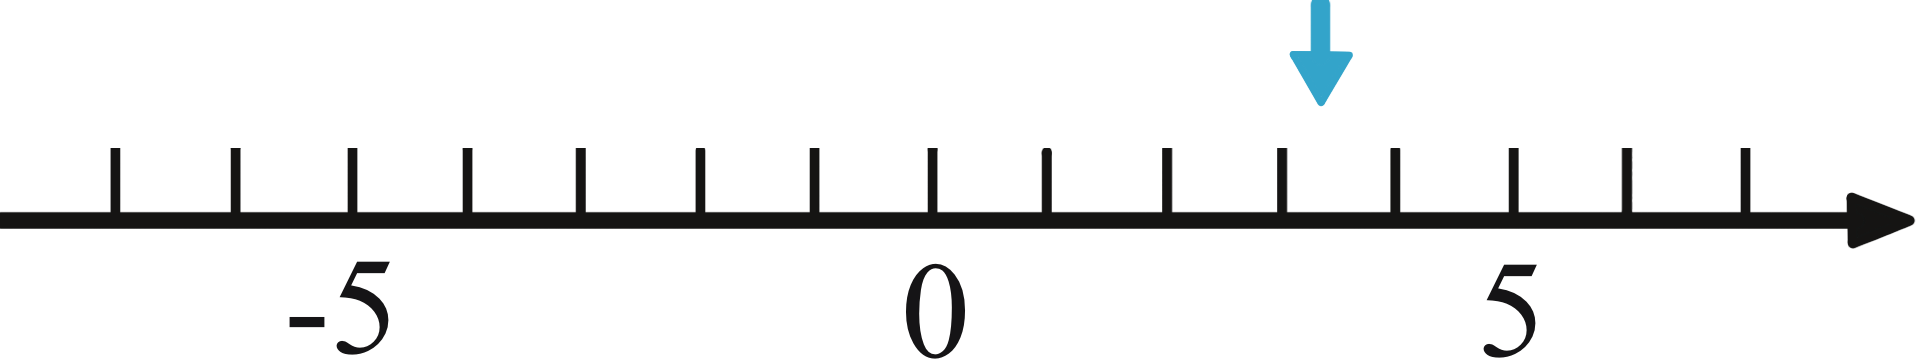
\includegraphics[width=\textwidth]{./ilustras-mat/Simulado_2-atividade_1.png}
\end{figure}

Qual dos racionais abaixo é um candidato para a posição da seta?


\begin{escolha}

  \item $\sqrt{3}$

  \item $\sqrt{5}$

  \item $\sqrt{6}$

  \item $\sqrt{10}$


\end{escolha}


\num{2} A idade estimada do universo é de cerca de 13,8 bilhões de anos. Essa
estimativa é baseada em dados observacionais e teóricos, incluindo a
radiação cósmica de fundo e a taxa de expansão do universo.
Acredita-se que o universo tenha se originado a partir de uma grande
explosão, conhecida como Big Bang, que ocorreu há cerca de 13,8
bilhões de anos. Desde então, o universo tem continuado a expandir-se
e a evoluir, dando origem a galáxias, estrelas e planetas, incluindo a
Terra. O estudo da idade do universo é fundamental para entendermos a
história e a evolução do cosmos.

A estimativa de idade do universo pode ser representada por:

\begin{escolha}

\item $138 \cdot 10^{6}$

\item $13,8 \cdot 10^{7}$

\item $1,38 \cdot 10^{10}$

\item $138.000.000$

\end{escolha}


\num{3} Quatro colegas pintaram uma parede. Jorge pintou $\frac{1}{6}$ dessa parede, Gabriel pintou $\frac{3}{18}$, Mário pintou $\frac{2}{8}$ e Lucas $\frac{3}{8}$.

\pagebreak
Quais deles pintaram a mesma quantidade?

\begin{escolha}

  \item Jorge e Mário.

  \item Gabriel e Lucas.

  \item Mário e Lucas.

  \item Jorge e Gabriel.

\end{escolha}

\num{4} Em uma loja de artigos esportivos, o preço das camisetas costuma 
subir em períodos como finais de campeonato ou em copas do Mundo. Um determinado
artigo teve o preço reajustado com aumento de 10\%, mas depois de algumas semanas
lançou-se a promoção que daria 10\% de desconto se fosse realizado o
pagamento por PIX.

Se o pagamento for realizado por PIX, durante o período promocional,
podemos afirmar que será pago:

\begin{enumerate}

\item o mesmo valor de antes do aumento.

\item valor 1\% maior do que antes do aumento.

\item valor 1\% menor do que antes do aumento.

\item valor 99\% menor em comparação com o preço depois do aumento.

\end{enumerate}


\num{5} O estacionamento de um shopping, cobra pela primeira hora, R\$ 8,00 e, em cada hora seguinte,
ou fração da hora, R\$ 3,00.

Uma pessoa que pagou 23 reais permaneceu com seu veículo no estacionamento por até:

\begin{escolha}
  
  \item 5 horas, porque $23 = 8 + 3x$.

  \item 3 horas, porque $23 = 8x - 3$.

  \item 6 horas, porque $23 = 8 + (x - 1) \cdot 3$.

  \item 5 horas, porque $23 = 3 + (x - 1) \cdot 3$.

\end{escolha}


\num{6} Analisando a sequência (1, 4, 9, 16, 25, \ldots{}), Carlos e Lucas 
ficaram muito curiosos descobrir um critério para continuar a sequência.

Após pensar muito Carlos e Lucas estabeleceram que os três os próximos
números são:

\begin{escolha}

  \item 35, 46 e 55.

  \item 36, 49 e 64.

  \item 30, 41 e 54.

  \item 41, 50, 59.

\end{escolha}

\pagebreak
\num{7} Uma empresa estimou que o custo de produção, em milhares de reais, de
n produtos de sua linha esportiva é calculado pela expressão $C(n)= n² - n + 10$.

Se o custo foi de 100 mil reais, então, o número de produtos produzidos foi

\begin{escolha}
  
  \item 6. 
  
  \item 7. 
  
  \item 8. 
  
  \item 10.

\end{escolha}

%Faltam as habilidades e o gabarito.}

\num{8} Mário gosta muito de montar e desmontar coisas. Recentemente ele 
ganhou dos pais um brinquedo de robótica e estava estudando as engrenagens
e seus movimentos. Ele percebeu que, enquanto a menor delas dá uma volta
completa, a maior gira só meia-volta.

\begin{figure}[htpb!]
\centering
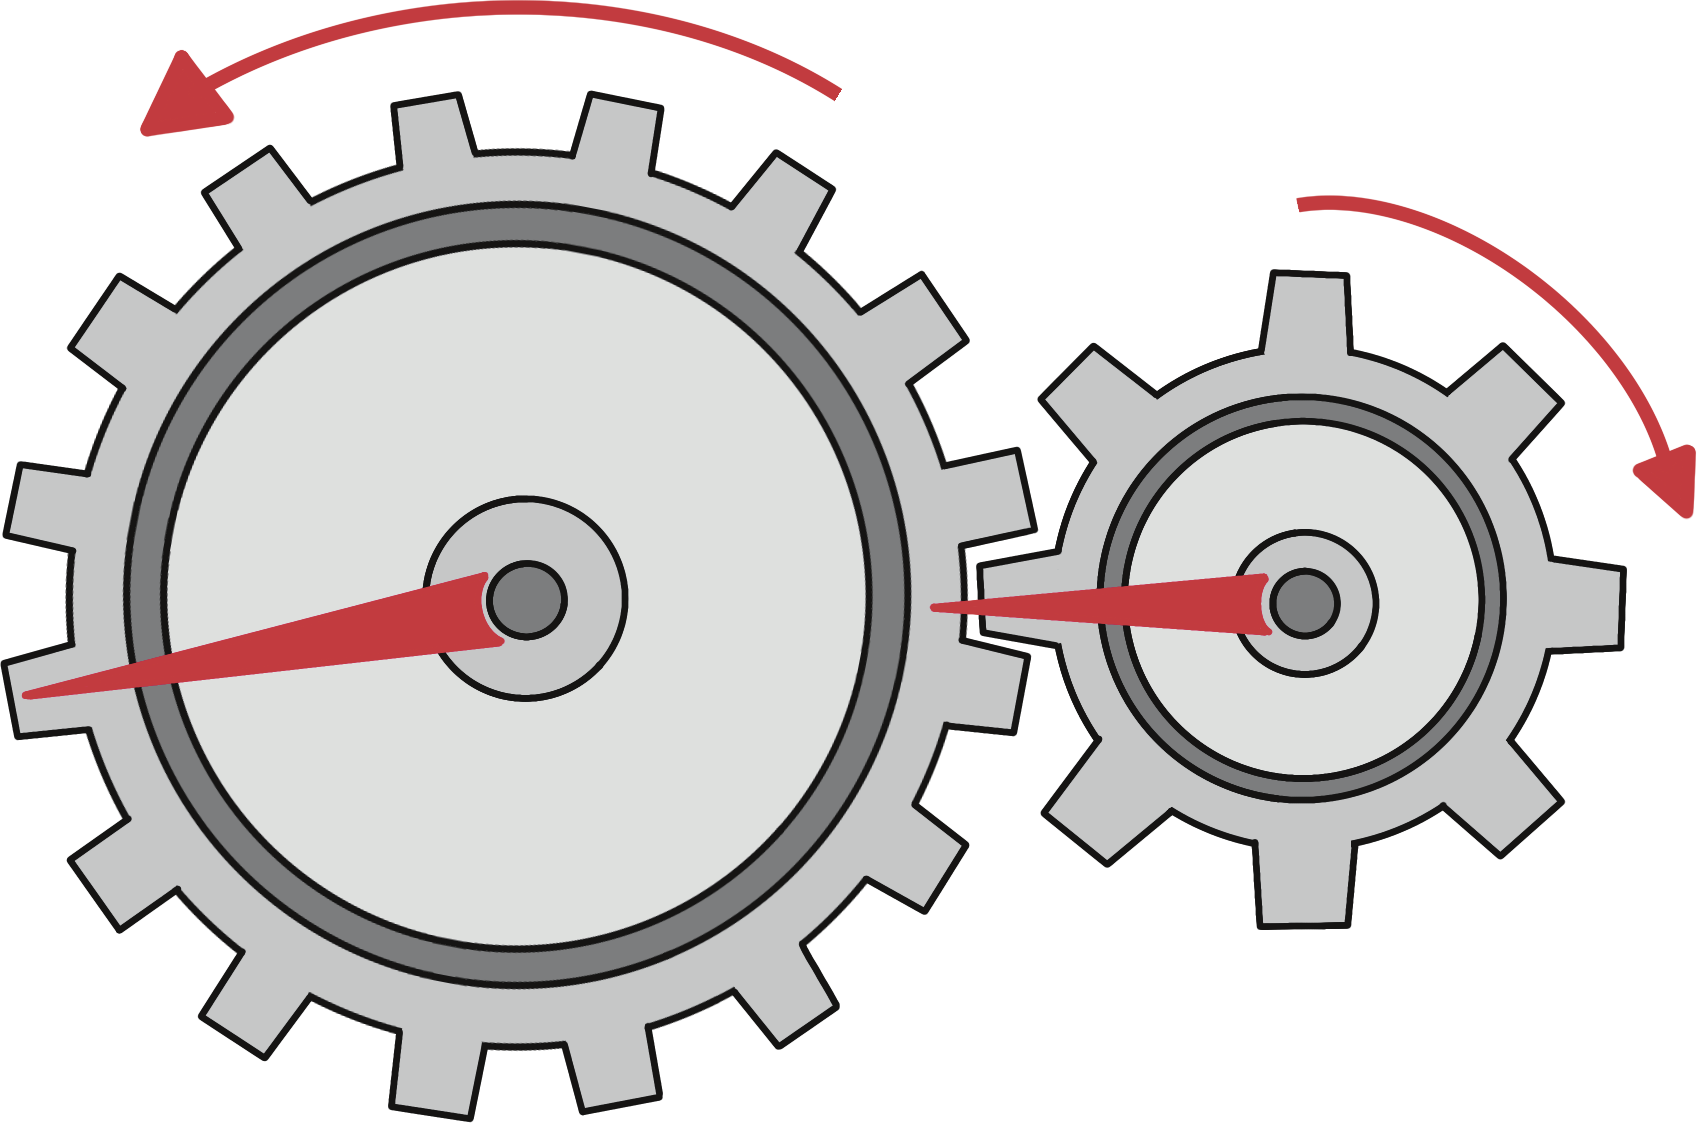
\includegraphics[width=.8\textwidth]{./ilustras-mat/Simulado_2-atividade_8.png}
\end{figure}

Quantas voltas dará a engrenagem grande, considerando que a engrenagem
pequena dará 20 voltas completas?

\begin{escolha}

  \item 20 voltas.

  \item 5 voltas.

  \item 10 voltas.

  \item 15 voltas.

\end{escolha}

\pagebreak

\num{9} Observando dois reservatórios A e B, percebeu-se que os volumes de 
cada um deles, em litros, variam em função do tempo \textbf{t}, medido em
minutos, de acordo com as seguintes relações:

$V_A = 400 + 4t$ e $V_B = 6000 - 4t$

Em que instante em que os reservatórios estarão com o mesmo volume?

\begin{escolha}

  \item t = 500 minutos

  \item t = 550 minutos

  \item t = 700 minutos

  \item t = 1 500 minutos

\end{escolha}

\num{10} Em um círculo de raio 12 está inscrito um quadrilátero ABCD.
Sobre a soma dos ângulos opostos BÂD e BCD %aqui precisamos colocar circunflexo em cima do C em BCD, mas não encontrei como fazer isso 
, podemos afirmar que vale:

\begin{escolha}

  \item 12 x 180°.

  \item 360°.

  \item 90°.

  \item 180°.

\end{escolha}



\num{11} Em uma experiência em uma aula de Matemática, o professor André
desafiou os alunos a descobrir a altura do mastro de uma bandeira. O aluno
que descobriu a altura fincou, paralelamente a esse mastro, um bastão de
1m. Medindo as sombras projetadas no chão pelo bastão e pelo mastro,
o aluno encontrou, respectivamente, 250 cm e 1250 cm. Portanto, a altura do
mastro, em metros, é

\begin{escolha}

  \item 5,0.

  \item 5,5.

  \item 6,0.

  \item 6,5.

\end{escolha}

\pagebreak
\num{12} O gráfico a seguir mostram o número de alunos que utilizaram
carros por aplicativo para ir à universidade, durante uma determinada
semana, de segunda a sexta-feira.

\begin{figure}[htpb!]
\centering
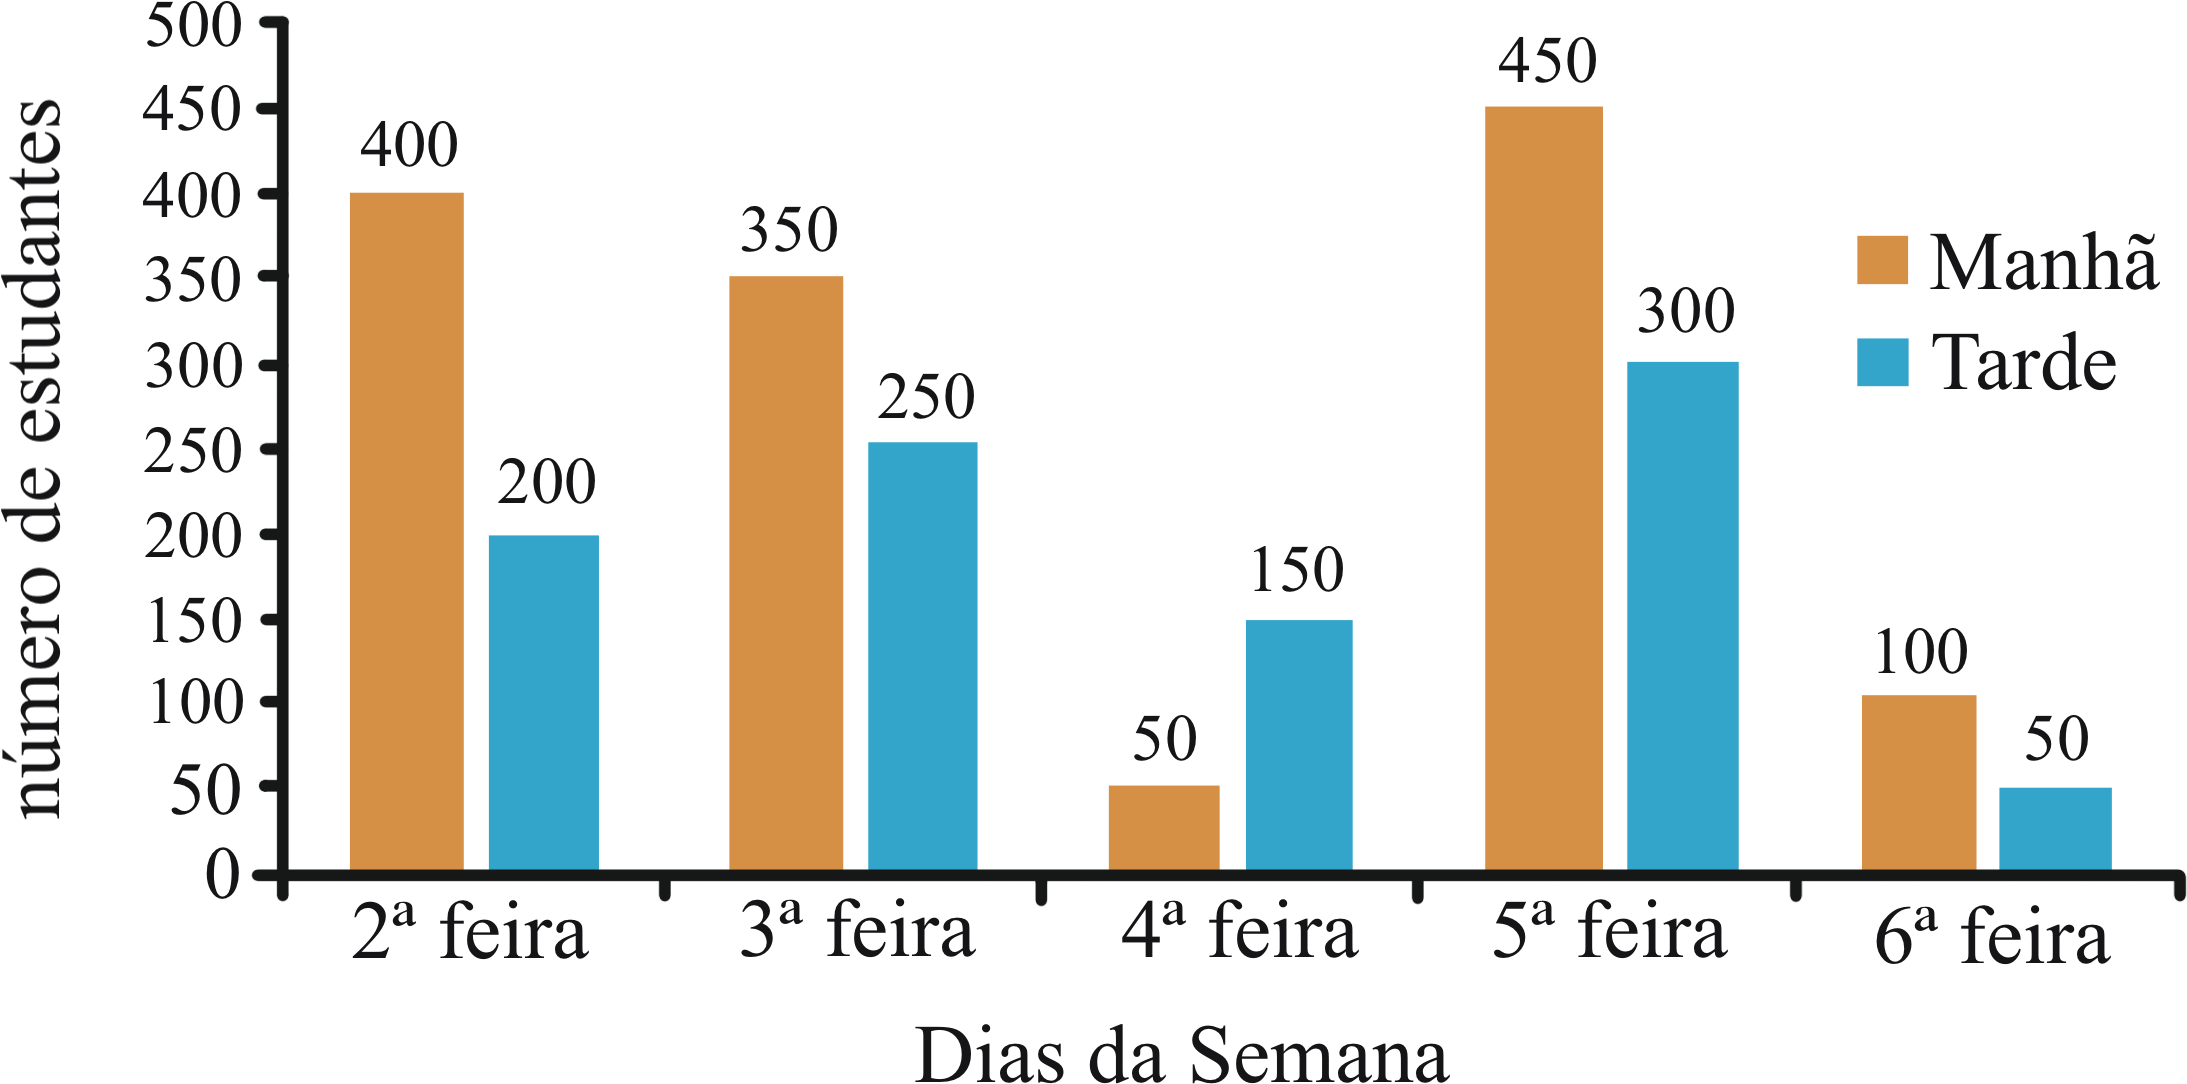
\includegraphics[width=\textwidth]{./ilustras-mat/Simulado_2-atividade_12.png}
\end{figure}

Naquela semana, uma determinada empresa cobrou valores fixos de corrida,
desconsiderando a extensão dos deslocamentos. O valor variava apenas de 
acordo com o horário de viagem: no período da manhã foram cobrados 
R\$ 10,00; no da tarde, R\$ 15,00. Qual foi a receita bruta do dia 
em que houve maior volume de atendimento?

\begin{escolha}

  \item R\$ 4.500,00

  \item R\$ 9.000,00

  \item R\$ 13.500,00

  \item R\$ 15.000.00

\end{escolha}


\num{13} Uma empresa de importação de cosméticos conta com 30 funcionários
com a seguinte distribuição salarial em reais.

\begin{longtable}[]{@{}ll@{}}
\toprule
Nº de funcionários & Salário em R\$\tabularnewline
\midrule
\endhead
10 & 2.000,00\tabularnewline
12 & 3.600,00\tabularnewline
5 & 4.000,00\tabularnewline
3 & 6.000,00\tabularnewline
\bottomrule
\end{longtable}

O diretor financeiro tem como objetivo reduzir o custo da folha de
pagamento, por isso propôs ao conselho que fossem realizadas demissões
na faixa salarial de R\$ 3.600,00. Com esse corte, pretende alcançar
mediana de R\$ 2.800,00.

\pagebreak
Quantos funcionários devem ser demitidos?

\begin{escolha}

  \item 8

  \item 11

  \item 9

  \item 10

\end{escolha}

\num{14} Em uma distribuidora de produtos, os funcionários ``juntam'' as
caixas de tal forma que se possa colocá-las sobre paletes e passar o
plástico filme em volta.

Observe a seguir o modelo que o funcionário da empilhadeira está
organizando. Ele precisa pegar os cubos A e fazer a pilha de caixas
conforme o bloco B.

Quantas caixas A são necessárias para montar B?

\begin{figure}[htpb!]
\centering
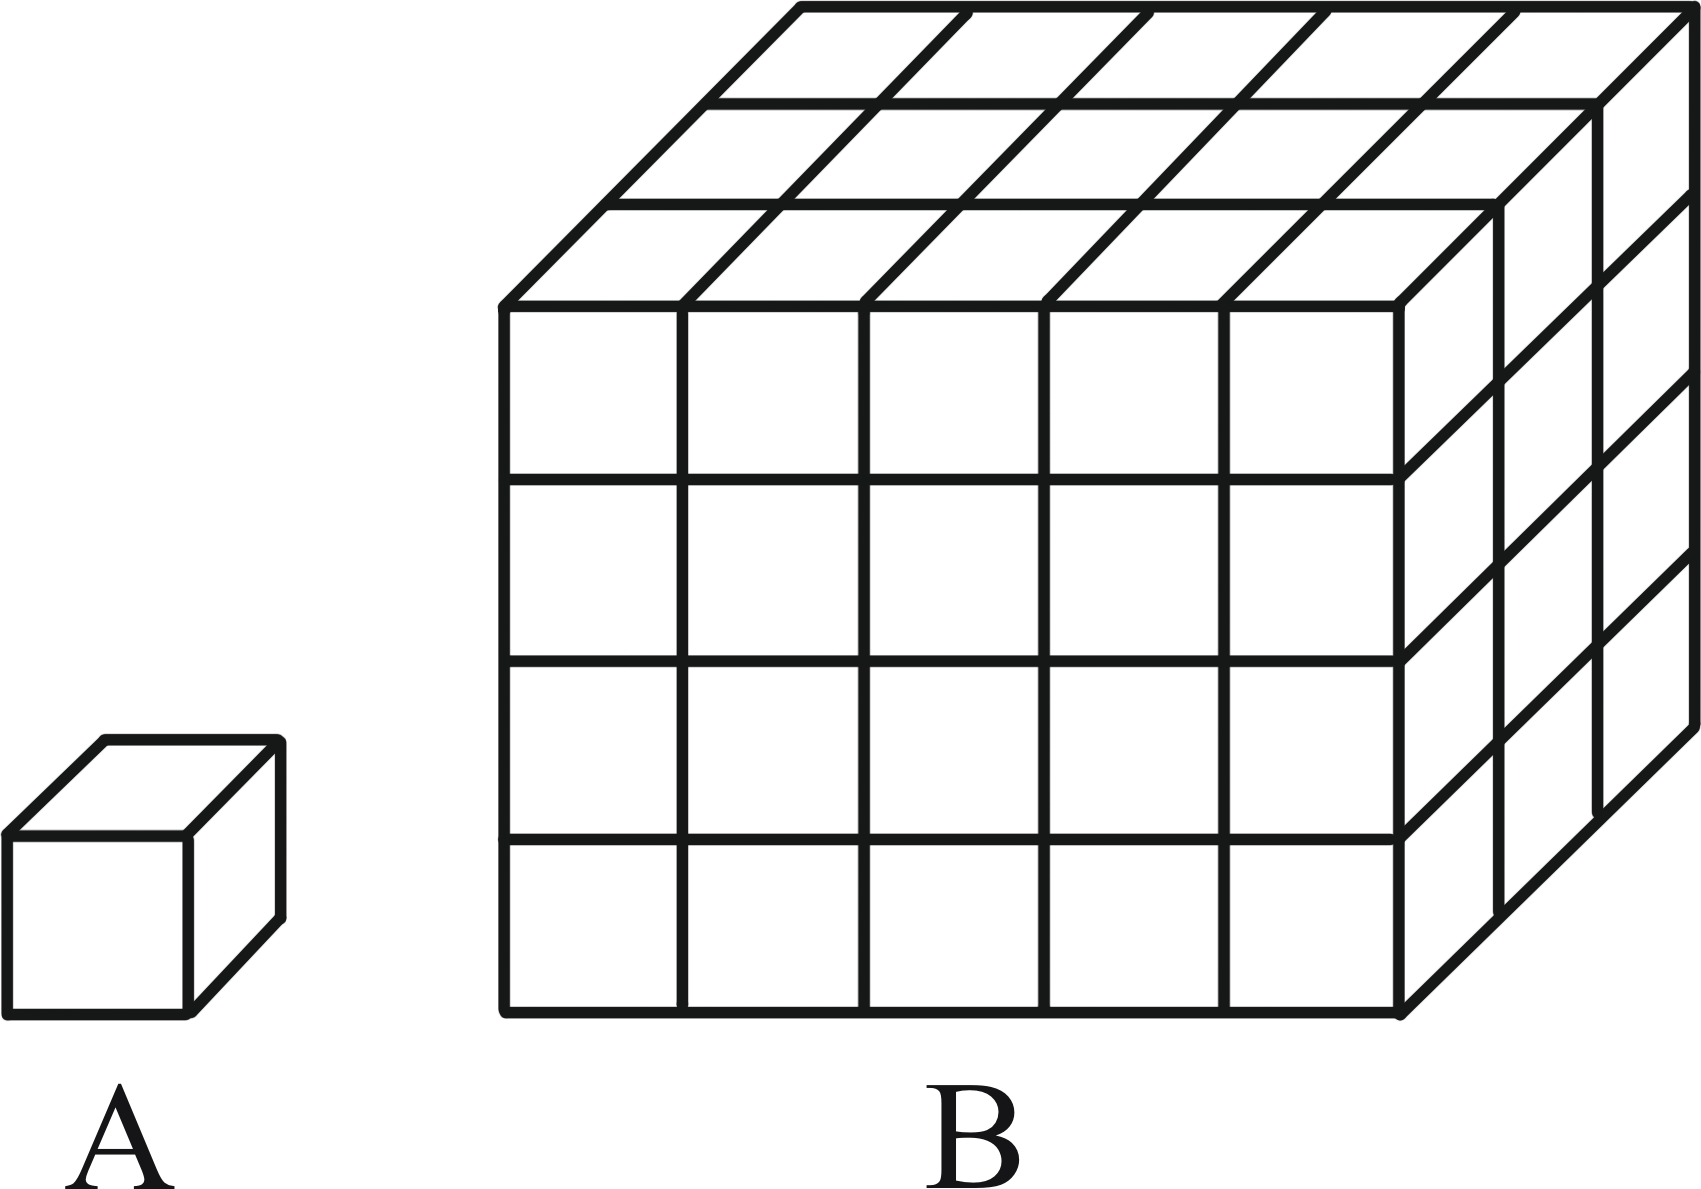
\includegraphics[width=.5\textwidth]{./ilustras-mat/Simulado_2-atividade_14.png}
\end{figure}

\begin{escolha}

  \item 60

  \item 47

  \item 94

  \item 48

\end{escolha}

\pagebreak
\num{15} Seja um triângulo retângulo, cujos catetos medem 6 e 8.

\begin{figure}[htpb!]
\centering
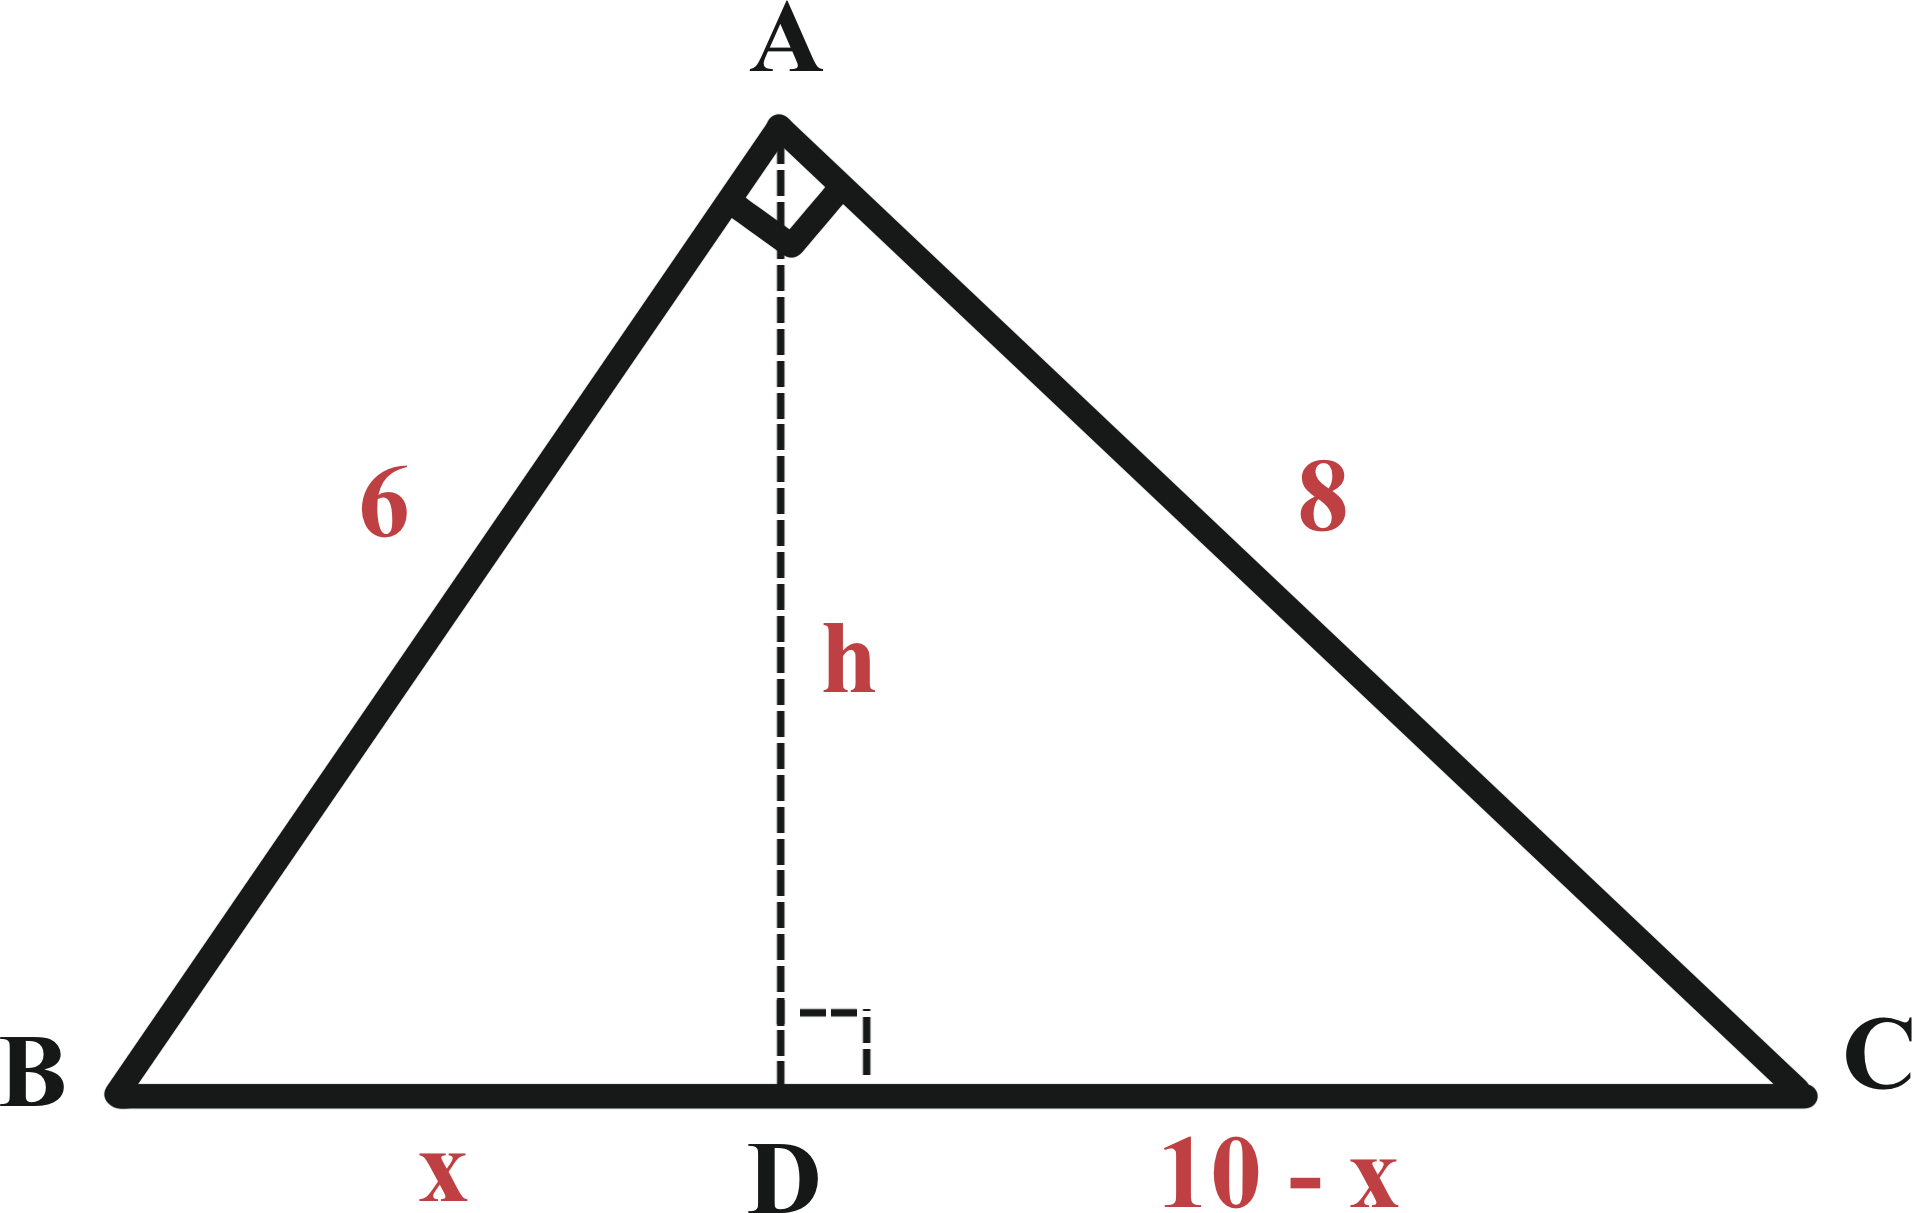
\includegraphics[width=.5\textwidth]{./ilustras-mat/Simulado_2-atividade_15_resposta.png}
\end{figure}

Qual a altura relativa à hipotenusa deste triângulo?

\begin{escolha}

  \item 3 cm

  \item 4 cm

  \item 4,8 cm

  \item 10 cm

\end{escolha}


\num{16} Leia o texto a seguir

\begin{quote}
O Ministério da Educação, por meio do Fundo Nacional de Desenvolvimento
da Educação (FNDE), tem liberado recursos para a construção de 6.116
quadras esportivas {[}...{]}

``Essa quadra foi um presente para a escola e para a comunidade'',
comemora a diretora Socorro Lima da Silva. Segundo ela, duas vezes por
semana alunos da Escola Municipal Walmik Sampaio de Albuquerque utilizam
a quadra da escola Vinícius de Morais para as aulas de educação física.
``Durante a semana, de 17h às 20h, a quadra é utilizada pela comunidade,
em jogos de futsal. E, nos fins de semana, é utilizada em atividades do
programa Escola Aberta, como eventos religiosos'', explica.

\fonte{ Ministério da
Educação. Escolas devem ser indicadas até setembro para ter quadras. Disponível em:
http://portal.mec.gov.br/ultimas-noticias/384-fnde-1801140772/18039-escolas-devem-ser-indicadas-ate-setembro-para-ter-quadras.
Acesso em: 12 abr. 2023.}
\end{quote}

Considerando as afirmações do texto, é possível inferir que a principal 
função da quadra da escola Vinícius de Morais é

\begin{escolha}
\item aumentar recursos financeiros da cidade.

\item incentivar a prática de esportes na comunidade.

\item promover competições oficiais de diferentes modalidades.

\item ampliar a frequência de eventos não esportivos.
\end{escolha}

\pagebreak
\num{17} Leia o texto a seguir:

\begin{quote}
Para os povos da Antiguidade, o manuseio da espada era fundamental,
tendo em vista as constantes guerras e batalhas travadas.~ {[}...{]}

A Federação Internacional de Esgrima só foi criada em 1913. O primeiro
Campeonato Mundial da modalidade aconteceu em 1921, em Paris. Mas a
história da esgrima nos Jogos Olímpicos começou antes. Já em Atenas--1896
houve provas do esporte. Desde então, a esgrima nunca deixou de estar
presente em uma edição das Olimpíadas.

\fonte{Esgrima. Rede do Esporte. Disponível em:
http://rededoesporte.gov.br/pt-br/megaeventos/olimpiadas/modalidades/esgrima-1.
Acesso em: 12 abr. 2023.}
\end{quote}

Considerando as afirmações do texto, é possível afirmar que a esgrima é
um esporte oficial porque essa prática

\begin{escolha}
\item ocorre desde a Antiguidade.

\item é regulada por órgãos oficiais.

\item originou-se em guerras.

\item requer uso de instrumento específico.
\end{escolha}

\num{18}  Leia a reportagem a seguir.

\begin{quote}
O Breaking Dance é um estilo que foi inserido recentemente entre as
modalidades das Olimpíadas e integrará os próximos jogos de Paris, na
França, em 2024. O tema vem movimentando as comunidades de danças
urbanas em todo o Brasil, esquentando o debate sobre a legitimidade do
Break como modalidade olímpica, tendo em vista ser considerado,
originalmente, um estilo de dança da cultura hip hop.

\fonte{Portal do Governo da Paraíba. Painel Funesc de dança traz debate
sobre o Break Dance nas Olimpíadas. Disponível em:
https://paraiba.pb.gov.br/noticias/painel-funesc-de-danca-traz-debate-sobre-o-break-dance-nas-olimpiadas.
Acesso em: 12 abr. 2023.}
\end{quote}

Com base no texto, é possível afirmar que o Breaking Dance

\begin{escolha}
\item deu origem à cultura hip hop.

\item tornou-se um esporte.

\item incentivou as competições de dança.

\item não pode ser chamado de dança urbana.
\end{escolha}

\pagebreak
\num{19}
  No século 18, um químico francês chamado Lavoisier realizava experimentos de combustão e calcinação utilizando balanças para medir
  seus produtos e reagentes a fim de garantir bons dados quantitativos. A
  partir das medições feitas por Lavoisier nesses experimentos, ele
  postulou o que chamamos de Lei de Lavoisier.

\fonte{Texto autoral.}

Identifique, dentre as alternativas, aquela que apresenta um outro nome para a Lei de Lavoisier e sua definição.

\begin{escolha}
\item
  Lei da Inércia. Toda matéria deve permanecer no estado em que se
  encontra até que uma força aja sobre ela.
\item
  Lei das proporções constantes. Toda substância apresenta uma proporção
  constante em sua composição.
\item
  Lei de Gay-Lussac. Em pressão e temperatura constantes, os volumes dos
  gases de uma reação têm entre si uma relação de números inteiros.
\item
  Lei de conservação das massas. Em um sistema fechado, a massa total dos
  reagentes é igual à massa total dos produtos.
\end{escolha}

\num{20}
  Um fungo aquático que já levou à extinção diversas espécies de
  anfíbios que têm parte ou todo o ciclo de vida na água ameaça também
  os sapos terrestres. Um grupo de pesquisadores apoiado pela FAPESP
  constatou na Mata Atlântica uma mortandade sem precedentes de sapinhos
  que se desenvolvem longe do ambiente aquático. Os anfíbios estavam
  infectados com altas cargas do fungo quitrídio (\emph{Batrachochytrium
  dendrobatidis}), causador da quitridiomicose. [...]

\fonte{André Julião. Agência Fapesp. Fungo aquático que já extinguiu diversas espécies de anfíbios ameaça agora sapos terrestres, diz estudo. Disponível em:
https://agencia.fapesp.br/fungo-aquatico-que-ja-extinguiu-diversas-especies-de-anfibios-ameaca-agora-sapos-terrestres-diz-estudo/36843/.
Acesso em: 23 fev. 2023.}

\pagebreak
Indique a alternativa que mostra uma possível consequência do declínio da população de anfíbios.

\begin{escolha}
\item Além da perda de biodiversidade, as relações dentro do ecossistema são afetadas, tendo em vista que anfíbios possuem diversas funções ecológicas, como o controle de insetos transmissores de doenças.

\item A rápida dispersão do fungo causador da quitridiomicose impede a evolução de outras espécies que habitam o ecossistema, tendo em vista a
necessidade de investir energia apenas na fuga.

\item As populações de anfíbios, que passam a maior parte do ciclo na terra,
não são afetadas pelo fungo; entretanto, são obrigadas a mudar sua
reprodução, que depende da água, para evitar os fungos.

\item A alta pressão exercida pelos fungos na população de anfíbios fará
com que sapos, rãs e pererecas se modifiquem para adquirir resistência ao patógeno.
\end{escolha}

\num{21}
\begin{quote}
Centenas de cientistas, 5 anos
de investigações, telescópios espalhados por oito lugares diferentes - assim de constrói um trabalho gigantesco. Graças a essa estrutura, um grupo de cientistas foi capaz de captar as primeiras imagens de um buraco negro localizado no centro da Via Láctea, a galáxia em que vivemos no planeta Terra. 
Com impressionantes quatro
milhões de vezes a massa do Sol, o objeto foi retratado pela primeira vez
em um esforço colaborativo de centenas de estudiosos, reunidos
no projeto~\emph{Event Horizon Telescope}~(EHT).

\fonte{Fonte de pesquisa: BBC News Brasil. Terra corre perigo com buraco negro 'monstruoso' no centro da Via Láctea? Disponível em:
https://www.bbc.com/portuguese/internacional-61440848. Acesso em:
24 fev. 2023.}
\end{quote}

Buracos negros causam fascínio por conta da sua magnitude e de seu potencial
perigo. Quais seriam as possíveis consequências para o nosso planeta
caso nossa galáxia se chocasse com outra?

\begin{escolha}
\item
  Toda a matéria da Terra se separaria em partículas minúsculas; além da mudança na
  noção de tempo, que dentro de um buraco negro é quase nula.
\item
  Por ser muito pequena a Terra passaria ilesa pelas proximidades de um
  buraco negro, sem ser engolida.
\item
  A força gravitacional da Terra deformaria o buraco negro, mas mesmo
  assim ela seria absorvida e sua matéria seria incorporada pelo próprio buraco.
\item
  A força gravitacional do buraco negro empurraria a Terra de tal forma
  que o planeta se chocaria em outro corpo celeste com muita velocidade.
\end{escolha}

